% ----------------------------------------------------------------------------
% Setup and configuration
% ----------------------------------------------------------------------------

\documentclass{article}
\usepackage[utf8]{inputenc}

% for serious mathematical typesetting, https://www.ctan.org/pkg/amsmath
\usepackage{amsmath}

% package to manage images and define images folder, https://ctan.org/pkg/graphicx
\usepackage{graphicx}
\graphicspath{{figures/}}

% create hyperlinks in the document and disable border, https://ctan.org/pkg/hyperref
\usepackage[hidelinks]{hyperref}

% bibliography package and references file, https://www.ctan.org/pkg/biblatex
\usepackage{biblatex}
\addbibresource{references.bib}

% ----------------------------------------------------------------------------
% Document
% ----------------------------------------------------------------------------

\title{Modeling Gas Effects in a Bubbling Fluidized Bed Reactor for Biomass Pyrolysis}
\author{Gavin M. Wiggins, ??}
\date{March 2020}

\begin{document}

\maketitle
\tableofcontents

\section*{Abstract}

Fast pyrolysis of biomass in a fluidized bed reactor is typically conducted in a nitrogen gas environment. Recycling product gas can improve the economics of operating such a system by reducing reliance on pure process streams.

\section{Introduction}

Fast pyrolysis is a versatile method for thermochemical conversion of solid biomass into liquid bio-oil which can be used for bio-fuel and high-value chemical production. Bio-oil is commonly generated in bubbling fluidized bed and circulating fluidized bed reactor systems in which biomass particles rapidly devolatilize in the absence of oxygen into mixtures of light gases, condensable bio-oil vapors, and solid char \cite{Bridgwater-1999, Bridgwater-2018a, Mohan-2006}. Since biomass pyrolysis normally occurs in a non-oxidizing environment, the fluidization gas (carrier gas) is often pure nitrogen \cite{Mohan-2006}. To maximize bio-oil yields, the reactor typically operates at temperatures near 500$^\circ$C and must maintain particle residence times up to 10 seconds and gas residence times less than 2 seconds \cite{Bridgwater-2018a}. Deviations from these conditions can result in significant production and quality penalties, therefore optimal reactor design and control become crucial to achieving commercially viable bio-oil production.

To improve the economic possibilities of biomass fast pyrolysis systems, char can be burned for process heat while recycled pyrolysis gas can assist with fluidization \cite{Bridgwater-1999, Mante-2012}. The major generated components of pyrolysis gas are CO, CO$_2$, CH$_4$, H$_2$, and other light hydrocarbons \cite{Asadullah-2008, Zhang-2011}. Several experiments investigated the effects of these gases on reactor conditions and pyrolysis yields \cite{Mante-2012, Mullen-2013, Zhang-2011} but modeling the effects of the different gases was not discussed.

There are several models available that investigate the hydrodynamics and conversion of biomass at fast pyrolysis conditions in fluidized bed reactors \cite{Papadikis-2010, Mellin-2014}. As is typical for biomass pyrolysis, these models assume the fluidization gas is pure nitrogen. The authors are not aware of any published models in the biomass pyrolysis literature that account for the effects of fluidization or carrier gas other than nitrogen.

This paper uses engineering correlations, reduced-order modeling techniques, and CFD simulations to investigate the effects of gas mixtures in a fluidized bed biomass pyrolysis reactor. The scope of this study is to evaluate different gas mixtures and there effects on the hydrodynamics and biomass conversion in fluidized bed reactors operating at fast pyrolysis conditions.

\section{Experimental apparatus}

The NREL 2FBR system thermochemically converts biomass particles at fast pyrolysis conditions. The system is comprised of a bubbling fluidized bed reactor for fast pyrolysis of woody biomass particles. This reactor is referred to as the ``pyrolyzer'' in this work. An overview of the system is shown in Figure \ref{fig:nrel-system}. Dimensions and typical operating conditions of the pyrolyzer are given in Figure \ref{fig:nrel-pyrolyzer}. More information about the NREL pyrolysis system is available elsewhere \cite{Howe-2015, Trendewicz-2015}.

\begin{figure}[ht]
    \centering
    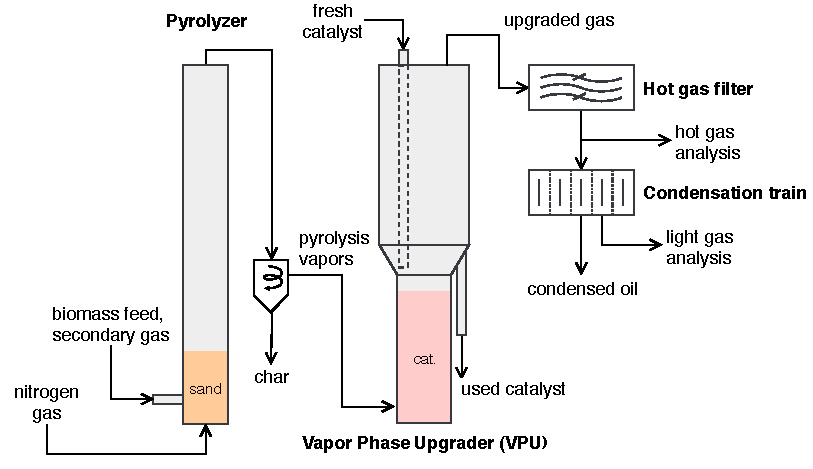
\includegraphics[width=\textwidth]{system.pdf}
    \caption{Overview of the NREL 2FBR system. Biomass fast pyrolysis occurs in the pyrolyzer (left) and gaseous products are catalytically upgraded in the vapor phase upgrader (right).}
    \label{fig:nrel-system}
\end{figure}

\begin{figure}[ht]
    \centering
    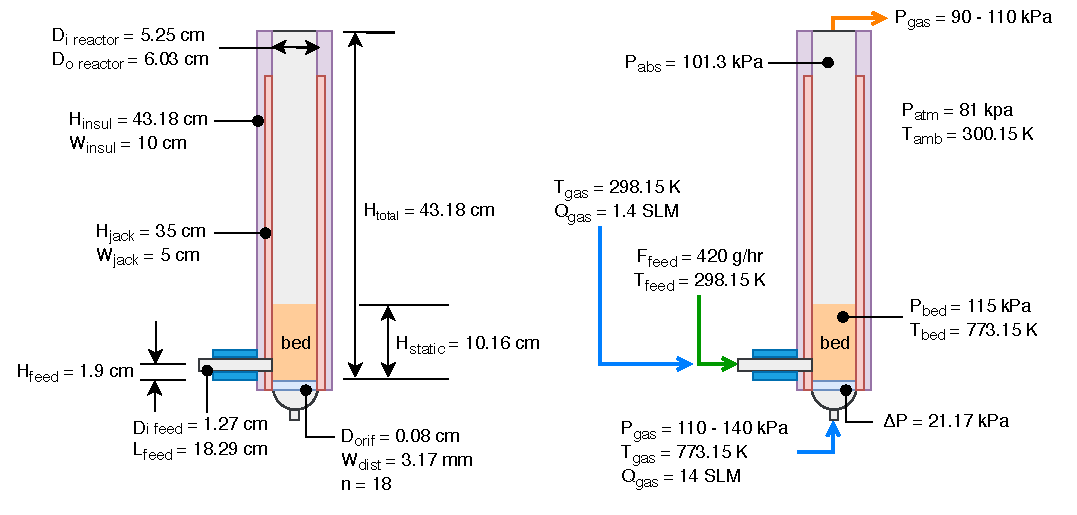
\includegraphics[width=\textwidth]{pyrolyzer.pdf}
    \caption{Dimensions and typical fast pyrolysis operating conditions of the NREL 2FBR pyrolyzer.}
    \label{fig:nrel-pyrolyzer}
\end{figure}

\section{Modeling approach}

Engineering correlations, reduced-order models, and CFD modeling techniques were used to investigate the effects of recycled gas on the operation of a fluidized-bed biomass pyrolysis reactor. The following sections discuss approaches implemented in this work for calculating gas properties and the associated effects on fluidization conditions and pyrolysis yields.

\subsection{Gas properties}

Density (kg/m$^3$) of an individual gas is calculated from the ideal gas law

\begin{equation}
    \rho_{gas} = \frac{P\;M}{R\;T}
\end{equation}

\noindent where P is pressure (Pa), M is molecular weight (g/mol), R is the gas constant [(m$^3$ Pa) / (K mol)], and T is temperature (K). Gas viscosity ($\mu$P) is given as

\begin{equation}
    \mu_{gas} = A + B\,T + C\,T^2 + D\,T^3
\end{equation}

\noindent where coefficients A, B, C, and D are obtained for a given gas from tables in Yaws' Handbook and T is gas temperature (K).

For a gas mixture, density is calculated as a weighted average of the individual gas densities. The viscosity of a gas mixture can be calculated from a variety of correlations.

\subsection{Fluidization correlations}

Here.

\subsection{CFD simulation}

Here.

\subsection{Pyrolysis kinetics}

Here.

\section{Model parameters}

Parameters for the reduced-order model and CFD simulations are provided in Table \ref{tab:params}. Biomass particle parameters and properties are representative of loblolly pine. Bed particle parameters are for typical sand material. Operating conditions and reactor dimensions are based on the previously discussed NREL 2FBR fluidized bed pyrolysis unit.

\begin{table}[ht]
    \centering
    \caption{Biomass, bed, and reactor modeling parameters. Particle diameters represent the Sauter-mean diameter.}
    \begin{tabular}{lll}
        \hline
        Parameter & Description & Value \\
        \hline
        d$_\textrm{p,\,bed}$    & diameter of bed particle          & 235 $\mu$m \\
        $\phi_\textrm{bed}$     & sphericity of bed particle        & 0.0 \\
        d$_\textrm{p,\,bio}$    & diameter of biomass particle      & 135 $\mu$m \\
        $\phi_\textrm{bio}$     & sphericity of biomass particle    & 0.0 \\
        $\rho_\textrm{bio}$     & density of biomass particle       & 540 kg/m$^3$ \\
        h$_\textrm{reactor}$    & reactor height                    & 43.18 cm \\
        h$_\textrm{static}$     & static bed height                 & 10.16 cm\\
        tk                      & reactor temperature               & 773 K \\
        \hline
    \end{tabular}
    \label{tab:params}
\end{table}

\section{Results and discussion}

Here.

\section{Conclusion}

Here.

\section{Open source code}

Python models used to generate results for this article are available on the CCPC GitHub at \url{https://github.com/ccpcode} in the X repository. Functionality provided by the Chemics package was used for gas properties and various fluidization calculations. See the Chemics documentation at \url{https://chemics.github.io} for more information.

\printbibliography

\end{document}
